\chapter{State of the Art}\label{chap:state-of-the-art}
This chapter presents the current stage of the technologies related to our application, specifically the different kinds of simulators that are currently present in the market (\sectionref{sec:assembly-simulators}), both specific to one architecture (\subsectionref{subsec:specific-assembly-simulators}) and architecture-agnostic simulators (\subsectionref{subsec:generic-assembly-simulators}).\\
Finally, it includes a comparison between all the mentioned simulators and our proposed application (\sectionref{sec:comparison}).



\section{Assembly simulators}\label{sec:assembly-simulators}
An `\gls{assembly simulator}' is a CPU simulator that enables the user to program it through an \gls{assembly}, and it usually has an educational purpose: either to aid the user in learning the language, or as an exercise for the programmer in order to give them a better understanding of CPU architecture and software development.

These simulators typically offer an interface that allows the user to execute the program step-by-step and see the current state of the simulated \gls{computer}.


\subsection{Specific simulators}\label{subsec:specific-assembly-simulators}
The vast majority of simulators that can be found today focus on emulating a specific \gls{ISA}, which can range from simple 8-bit microprocessors like the Intel 8080\supercite{i8080emulator} to architectures that are used today, like \gls{ARM} Thumb\supercite{QtARMSim}.

\noindent
Here, we'll focus on two examples: \hyperref[subsubsec:kite]{Kite} and \hyperref[subsubsec:armlite]{ARMLite}.


\subsubsection*{Kite}\label{subsubsec:kite}
Kite\supercite{song_kite2019} is a simulator that models a five-stage \gls{pipeline} \gls{RISC-V} CPU, based on the model described in \textit{Computer organization and design: the hardware/software interface (RISC-V edition)}\supercite{PattersonDavidA.2018Coad}, by D. Patterson and J. Hennessy, and implemented in C/C++. It was developed in 2019 in order to provide students of Yonsei University (Seoul, Korea) with an easy-to use simulator to accompany follow its Computer Architecture course.

It incorporates advanced features derived from a \gls{pipeline} architecture, such as \gls{instruction dependency} detection and \gls{pipeline stalls}, among others. These `under the hood' features offer a better understanding of the underlying concepts of computer architecture.

The simulator consists of an executable with a \gls{CLI} that takes three input files: the program's code, the register's state, and the data \gls{memory}'s state. It loads the state of registers and data \gls{memory}, executes the program's code and saves the state to the specified files, after the execution, printing some statistics (Figure \ref{fig:kite}). It also implements a \gls{debug} mode that prints the state of each instruction on the \gls{pipeline}, each \gls{clock cycle}.

\begin{figure}[h]
  \caption{Kite simulator \gls{CLI}.}
  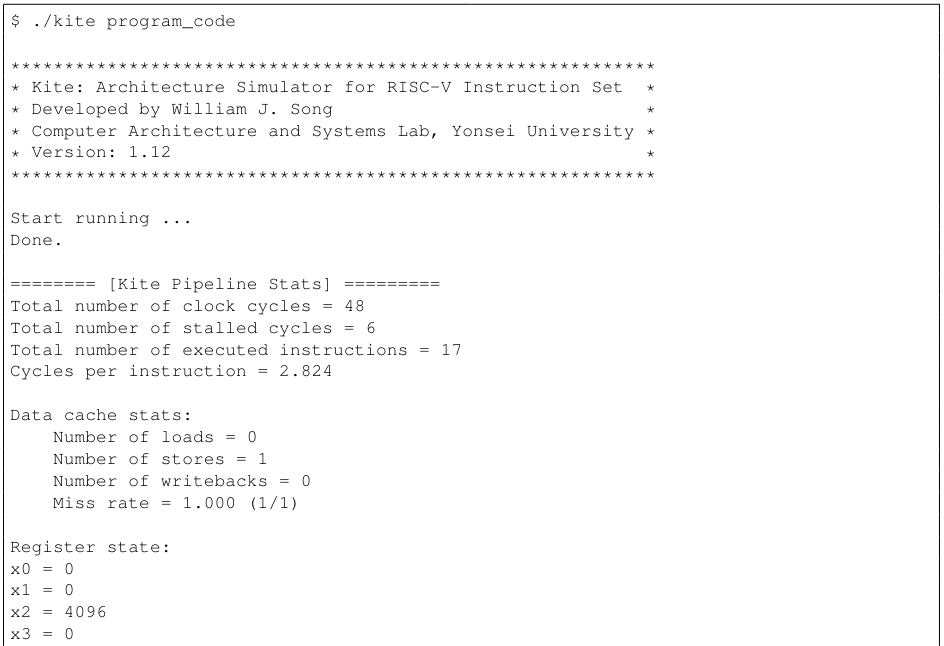
\includegraphics[width=0.7\textwidth]{kite.png}
  \label{fig:kite}
\end{figure}

Its source code can be found in the Yonsei University Computer Architecture and Systems Lab's GitHub\supercite{kiteGH}.


\subsection*{ARMLite}\label{subsubsec:armlite}
ARMLite\supercite{ARMLite} is a web-based simulator for a 32-bit `\glsdisp{ARM}{ARM-like}' processor. It includes a basic set of instructions described in \textit{Assembly Language Programming}\supercite{PawsonRichard.2020Ass}, by R. Pawson. This simulator was developed for educational purposes, but specifically to target AQA\supercite{AQA}'s Assembly language instruction set for its A-level computer syllabus\supercite{AQAInstructionSet}.

The simulator offers a \gls{GUI} (Figure \ref{fig:armlite}) that shows the current state of the \glspl{register} and the data \gls{memory}, as well as the current instruction and the status bits. It also adds \gls{I/O} support (a text box and a display), and options to start, stop, pause, resume, and slow or speed up execution, as well as step-by-step execution. It allows for users to load, save, and edit their programs, as well as a box to output system information (errors, last action performed, etc.).

\begin{figure}[h]
  \caption{ARMLite executing Conway's Game of Life\normalfont\supercite{Gardner1970fantastic}.}
  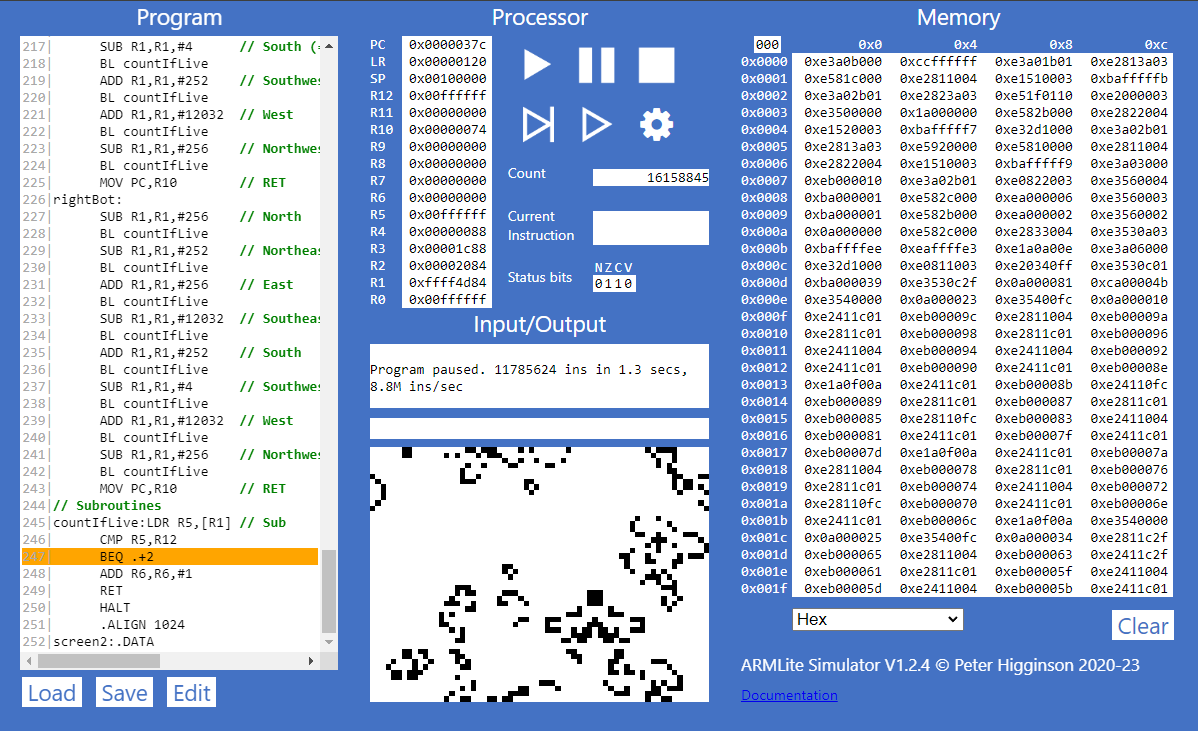
\includegraphics[width=0.7\textwidth]{ARMLite.png}
  \label{fig:armlite}
\end{figure}

While not being \gls{FOSS} \textit{per se} (we couldn't find any information about the license used by this simulator), the simulator uses JavaScript, which means the browser interprets the webpages's source code locally. As the code is \glsdisp{obfuscate}{unobfuscated} and is, to date, public and free to use, we \textit{could} consider this simulator \gls{FOSS}.



\subsection{Generic simulators}\label{subsec:generic-assembly-simulators}
We consider simulators that are able to define and execute multiple \glspl{ISA} `generic simulators'. They add a significant complexity to those types of simulators, due to the fact that they must be able to dynamically adapt to the different architectures.

Two different approaches to creating such simulators can be found in two specific examples: \hyperref[subsubsec:sail]{Sail} and \hyperref[subsubsec:creator]{CREATOR}.


\subsubsection*{Sail}\label{subsubsec:sail}
Sail\supercite{sail} is an \gls{ISA} definition language. It was developed by the Rigorous Engineering of Mainstream Systems (REMS)\supercite{rems} research group, from the University of Cambridge, as a tool to allow \glspl{ISA} to be mathematically modeled and verified and formally proven\supercite{ArmstrongAlasdair2019IsfA}.

This tool can not only type-check instruction and vector lengths for the \gls{ISA}, generate \glspl{theorem prover} definitions of the architecture and tests, or automatically generate documentation, but, more importantly for our specific case, it can generate executable simulators in C or OCaml based on those \glspl{ISA}.


\subsubsection*{CREATOR}\label{subsubsec:creator}
CREATOR\supercite{creator} is a web-based didactic and generic \gls{assembly} simulator. It was created by the ARCOS group from Universidad Carlos III de Madrid as a tool to teach students from the Computer Architecture and Computer Structure courses \gls{assembly} programming\supercite{creatorZenodo}.

It is a fully-fledged simulator, with support for an \gls{assembly} editor with syntax highlighting and error detection, step-by-step execution, \gls{I/O}, breakpoints, visualization of \gls{memory}, \glspl{register} and \gls{stack}, floating point support, loading and saving files, adding libraries, detection of argument passing conventions, etc., all accessible through its \gls{GUI} (Figure \ref{fig:creator}). 

Furthermore, it allows the user to view, edit, and create the architecture in use, using JavaScript. CREATOR allows the user to tweak and control a lot of the simulator's architecture and behavior. They can edit the \gls{memory} layout, register file (including number of bits, names and alias, and properties such as enabling reading or writing, if its value is saved when jumping into a \gls{subroutine}, which one is the stack and global pointer), \glspl{instruction} and \glspl{pseudo-instruction} (\glspl{clock cycle}, number of words, fields, etc.), and \glspl{directive}.


\begin{figure}[h]
  \caption{CREATOR's main \gls{GUI}.}
  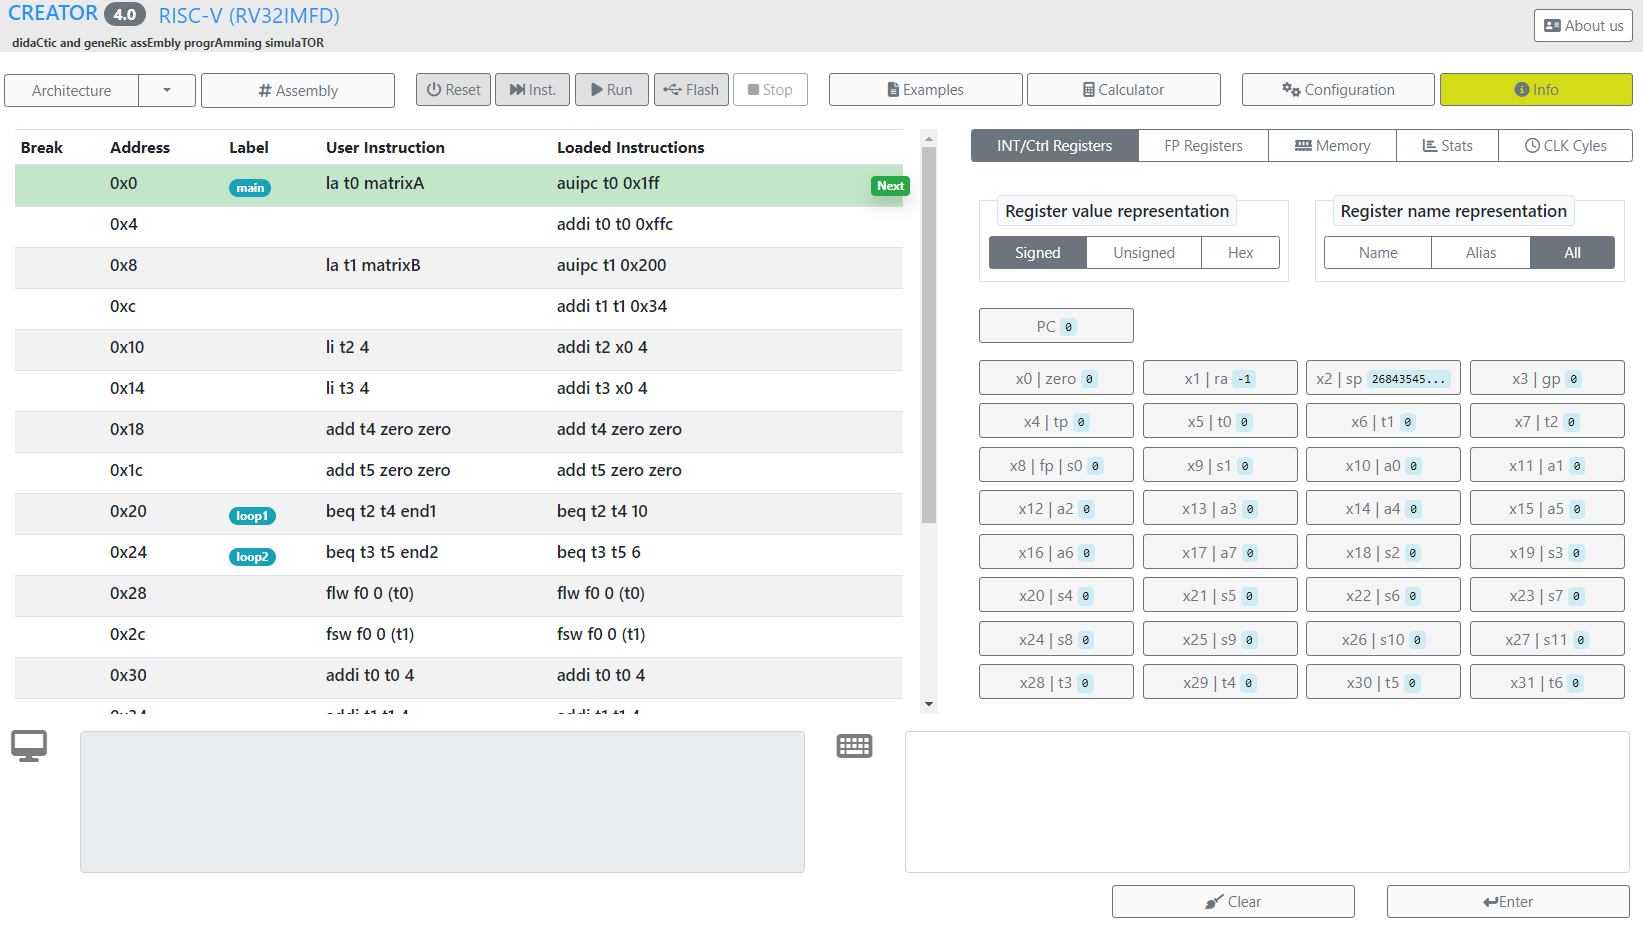
\includegraphics[width=0.7\textwidth]{creator.png}
  \label{fig:creator}
\end{figure}



\section{Comparison}\label{sec:comparison}
Our proposal aims to take the desirable features from each of the different simulators presented in order to create an application which fits our needs.

As we've justified before, we want a \textit{generic} simulator, and from the two discussed approaches we think \hyperref[subsubsec:creator]{CREATOR}'s approach is more suitable for our proposal, as the ability to quickly modify the architecture instead of \glsdisp{compilation}{re-compiling} the whole simulator encourages experimentation (less `friction'). We also must take into account that some features that make the simulator more generic might also create more of this `friction'; giving users a more fine-grained control over the architecture could discourage experimentation and add unnecessary complexity, if we prioritize for the user to understand \gls{assembly} over understanding computer architecture.  % TODO: citation needed

% Specific simulators...  % TODO

In Table \ref{tab:comparison}, we show a comparison of the different features of the current assembly simulators and our proposal.

\begin{table}[h]
  \caption{Feature comparison of current assembly simulators.}
  \label{tab:comparison}
  \begin{adjustbox}{max width=\textwidth}  % fit to textwidth
    \begin{threeparttable}[h]
      \begin{tabular}{>{\bfseries}lccccc}
          \toprule
          Simulator   & Kite       & ARMLite    & Sail       & CREATOR    & Proposal\\
          \hline
          Language    & C/C++      & JavaScript & OCaml      & JavaScript & C++23\\
          License     &BSD-3-Clause& None       &BSD-2-Clause& LGPLv2.1   & GPLv3\\
          % Architecture definition
          %             &            &            & \checkmark\tnote{a}
          %                                                  & \checkmark & \checkmark\\
          \gls{CLI}   & \checkmark &            &            & \checkmark & \checkmark\\
          \gls{I/O}   &            & \checkmark &            & \checkmark & \checkmark\\
          Step-by-step execution
                      &            &            &            & \checkmark & \checkmark\\
          Simple architecture definition
                      &            &            &            & \checkmark & \checkmark\\
          Native execution
                      & \checkmark &            & \checkmark &            & \checkmark\\
          In-browser  &            & \checkmark &            & \checkmark & \checkmark\tnote{*}\\
          \gls{GUI}   &            & \checkmark &            & \checkmark & \checkmark\tnote{*}\\
          Breakpoints &            & \checkmark &            & \checkmark & \checkmark\tnote{*}\\
          Architecture validation
                      &            &            & \checkmark &            & \checkmark\tnote{*}\\
          \bottomrule
      \end{tabular}
      \begin{tablenotes}
        \item [*] Future work.
        \item [a] Simulator needs to be \glsdisp{compilation}{recompiled} for any new architecture.
      \end{tablenotes}
    \end{threeparttable}
  \end{adjustbox}
\end{table}


We can also compare the mentioned simulators by plotting them on a two-dimension map (Figure \ref{fig:simulator_map}), with one axis representing how `generic' it is and the other one representing how `didactic' it is.

\drawiosvgfigure[0.5]{simulator_map}{Simulator comparison map.}
